%# -*- coding:utf-8 -*-
\section{Experiments and Results}
\label{sec6_2}

\subsection{Data and Experimental Setup}

The vasculature surface models were generated by applying the approaches proposed in \cite{Yang2014ICRA} from the original CTA images.
The resolution of the original data was $0.4 \times 0.4 \times 0.6 \text{mm}^3$.
For the sake of simplicity, only a segment of the abdominal aorta is depicted in this paper to demonstrate the effectiveness of our approach (see Fig. \ref{fig:VOI}).
The approach can be ported in order to process the model surfaces of the whole vasculature related to the surgical procedure to be simulated.

All of our experimental programs ran on a desktop machine equipped with Intel's 2.83GHz Core 2 Quad CPU and 4GB RAM.

\begin{figure}[t]
\centering
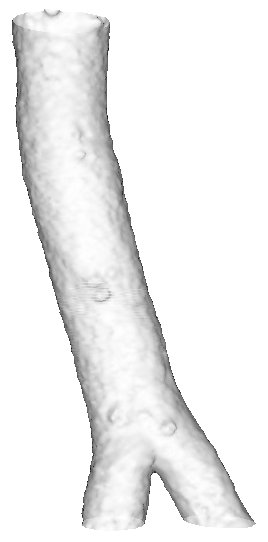
\includegraphics[height=2.0in]{Figures/chap06/original.png}
\caption{VOI-extracted surface model consisting of $74307$ polygons.}
\label{fig:VOI}
\end{figure}

\subsection{Validating Connectivity Between Vertices}

First of all, the polygonal elements in the patient-specific surface model of the human vessels need to be checked such that the connectivity between any pair of vertices are validated. %
After doing this, the integration of the model surface is guaranteed that the excessive polygons are kicked off.
Table \ref{tbl:Connectivity} shows that the total number of the polygonal surfaces were not changed, which implies that the given model (i.e., the local one) was already the largest-connected region in the model before the validation process. %

\subsection{Smoothing Model Surface}

Since the unavoidable noises introduced in the phase of image acquisition and processing, uneven surfaces may be found in the surface rendered based on the imagery.
The mess of artifacts and crusts may induce the problems in the smoothness of the delivery of the virtual surgical tools, e.g., guidewires, catheters, etc.
To avoid this situation, a thorough smoothing process is needed on the inner surface of the model, which is equivalent to the smoothing on the model surface per se.
\begin{table}[t]
\renewcommand{\arraystretch}{1.3}
\caption{Numbers of polygons before and after connectivity validation}
\label{tbl:Connectivity}
\centering
\begin{tabular}
{@{}l||r@{}}
%{@{}llrr@{}}
%\toprule
\hline
~                       & No. of polygons \\
\hline\hline
Before validation       & $74,307$  \\
After validation        & $74,307$  \\
\hline
\end{tabular}
\end{table}

The algorithm utilized in this processing task is implemented based on the low-pass filtering principles, with two parameters to be tuned in control of the smoothing effect on the objects. %
One of the parameters regulates the number of iterations the algorithm should take.
It is equivalent to the order of the polynomial that approximating the windowed sinc function given in (\ref{eqn:Approximation}).
The other parameter is used to configure the bandwidth of this so-called low-pass filter.

In this work, several parameter sets were given with the aim of searching for the one that can generate the most acceptable results.
The numbers of iterations of the smoothing were chosen to be $30$, $60$, and $100$ in the two cases, where the bandwidths were $0.1$, and $0.01$.

Judging from the resultant models in Fig. \ref{fig:Smooth}, the ones on the top row (see Figures \ref{fig:Smooth30-1}, \ref{fig:Smooth60-1}, and \ref{fig:Smooth100-1}) smoothed with the bandwidth $0.1$ are still fairly rough compared to the input, while the ones on the bottom row (see Figures \ref{fig:Smooth30-01}, \ref{fig:Smooth60-01}, and \ref{fig:Smooth100-01}) with the bandwidth $0.01$ are much better. %
With the increase of the number of iterations, the smoothing effect became more apparent, compared with the column of results from the one on its left.
At this stage of processing, we chose the parameter set which was used to generated the results depicted in Fig. \ref{fig:Smooth100-01} ($\text{no. of iterations} = 100$, $\text{pass band} = 0.01$). %
\begin{figure}[t]
\centering
\subfloat[]{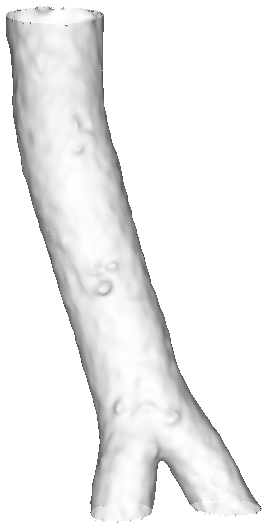
\includegraphics[height=2.0in]{Figures/chap06/smooth_30_1.png}%
\label{fig:Smooth30-1}}
\hfil
\subfloat[]{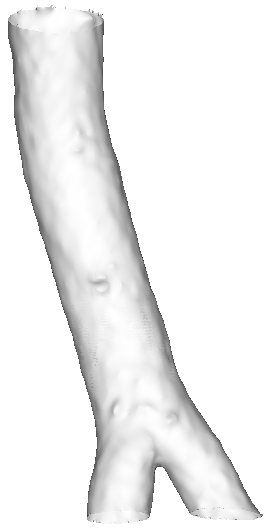
\includegraphics[height=2.0in]{Figures/chap06/smooth_60_1.png}%
\label{fig:Smooth60-1}}
\hfil
\subfloat[]{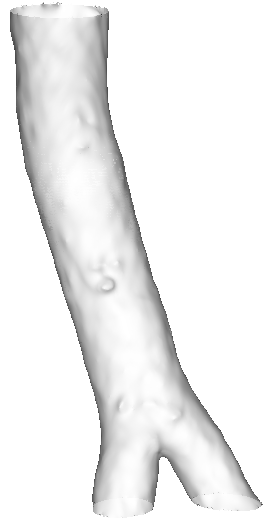
\includegraphics[height=2.0in]{Figures/chap06/smooth_100_1.png}%
\label{fig:Smooth100-1}}
\hfil
\subfloat[]{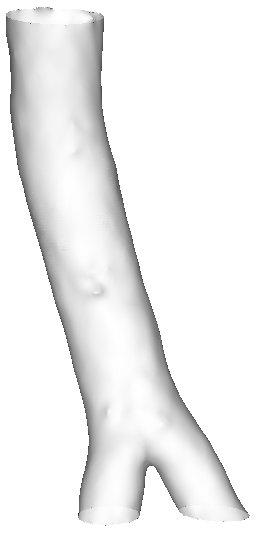
\includegraphics[height=2.0in]{Figures/chap06/smooth_30_01.png}%
\label{fig:Smooth30-01}}
\hfil
\subfloat[]{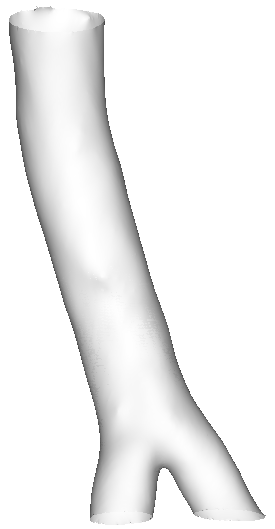
\includegraphics[height=2.0in]{Figures/chap06/smooth_60_01.png}%
\label{fig:Smooth60-01}}
\hfil
\subfloat[]{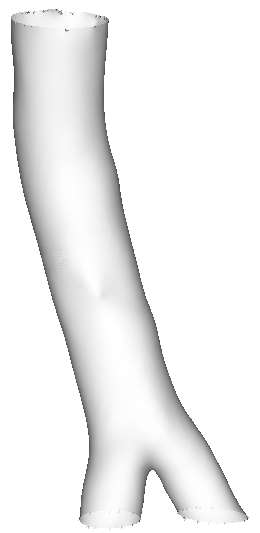
\includegraphics[height=2.0in]{Figures/chap06/smooth_100_01.png}%
\label{fig:Smooth100-01}}
\caption{Smoothing effects by applying different parameters: top row illustrate the results with $\text{pass band} = 0.1$, and the numbers of iterations are: $30$, $60$, and $100$, respectively; bottom row illustrate the results with $\text{pass band} = 0.01$, and the numbers of iterations are: $30$, $60$, and $100$, respectively.}%
\label{fig:Smooth}
\end{figure}

\subsection{Elimination of Component Polygons}

The elimination of polygon elements of the model surface was conducted after the smoothing computation terminated demonstrated in the last section.

For the input surface model, over $74$k polygons were required to model the vessel segment by using Marching Cubes method \cite{Lorensen1987MC}.
One can imagine that the overall number of the polygons needed to model the whole aorta and the trees of the coronary arteries.
Rendering the large amount of data will surely exhaust the most memory on any machine with typical hardware configuration, thus no sufficient space could be spared for the interaction and other computation.
To facilitate this situation, we adopted the decimation algorithm introduced in Section \ref{subsec:decimation} with multiple sets of parameters in a series of experiments. %

In this work, the termination conditions of the adopted algorithm were set to $10\%$, $50\%$, $75\%$, $90\%$, and $99\%$, respectively.
By termination condition, which is equivalent to the reduction rate, we mean that the rate of the total number of the polygonal elements deleted with respect to the total number of the polygonal elements in the input model surface. %
This can be written as follows
\begin{equation}
\label{eqn:ReductionRate}
\text{Reduction Rate (\%)} = \frac{\text{No. of \emph{deleted} Polygons}}{\text{No. of Input Polygons}}.
\end{equation}

Table \ref{tbl:Decimate} illustrates the effects of the decimation algorithm.
Figure \ref{fig:Decimate} depicts the visualization results of the decimation with typical parameters.
Observing the results, visualization in Figures \ref{fig:Decimate90} and \ref{fig:Decimate99} contain acceptable amounts of polygons.
However, the visualization in fig. \ref{fig:Decimate99} unveiled obvious alterations in its geometry.

\subsection{Discussions}

All the programs ran in the experiments were written in C++.
Some of the functioning modules were implemented based on the Visualization Toolkit (VTK) \cite{Schroeder2000VTK}, an open source effort containing various of computation facilities implementing algorithms from both the general and special fields of computer graphics. %

In validating the connectivity of the adjacent points among the surface model, the algorithm was configured to extract the largest-connected areas in this work.
To depress the effects from the noisy meshes introduced by image processing, a surface smoothing algorithm was employed to remove these meshes by slightly altering the locations of the vertices of the meshes. %
In smoothing the surface, two distinct parameters were the key switches for the algorithm, among which the width of the pass band of the low-pass filter and the number of the iterations to be performed were determined. %
Between the number of iterations and the smoothing effects on the surface, a positive correlation was demonstrated that the larger the number, the smoother the result.
On the other hand, the width of the pass band and the smoothing effects implied a negative correlation that the narrower the pass band, the smoother the result.
%One thing to be noted is that the loss of certain details occurred on all the resultant surface models.
\begin{table}[t]
\renewcommand{\arraystretch}{1.3}
\caption{Reduction rates and quantities of polygons in the model surface after decimation}
\label{tbl:Decimate}
\centering
\begin{tabular}{c||r r r r r}
\hline
%\bfseries      & \bfseries Quantity of polygonal surfaces \\
Reduction Rate ($\%$)  &    $10$ &    $50$ &    $75$ &   $90$ &  $99$ \\
\hline\hline
No. of Polygons & $66875$ & $37153$ & $18576$ & $7430$ & $743$ \\
\hline
\end{tabular}
\end{table}
\begin{figure}[t]
\centering
\subfloat[]{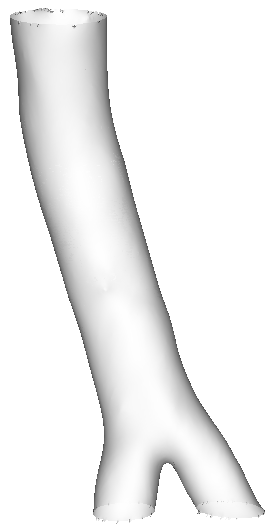
\includegraphics[height=2.0in]{Figures/chap06/smooth_100_01_d10.png}%
\label{fig:Decimate10}}
\hfil
\subfloat[]{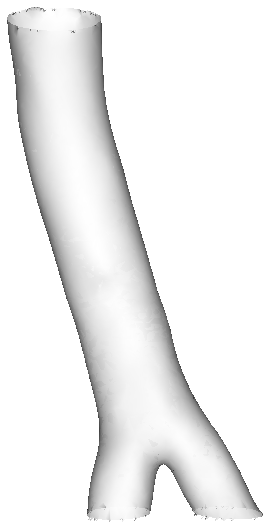
\includegraphics[height=2.0in]{Figures/chap06/smooth_100_01_d90.png}%
\label{fig:Decimate90}}
\hfil
\subfloat[]{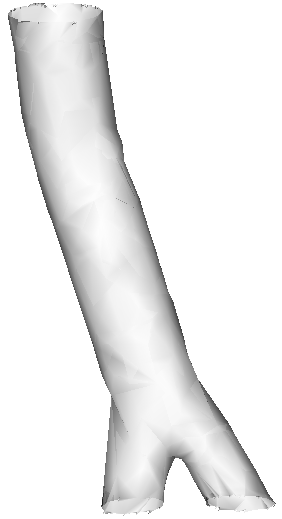
\includegraphics[height=2.0in]{Figures/chap06/smooth_100_01_d99.png}%
\label{fig:Decimate99}}
\hfil
\subfloat[]{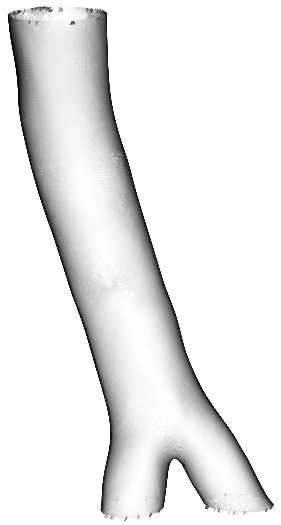
\includegraphics[height=2.0in]{Figures/chap06/smooth_100_01_d10_w.png}%
\label{fig:Decimate10-w}}
\hfil
\subfloat[]{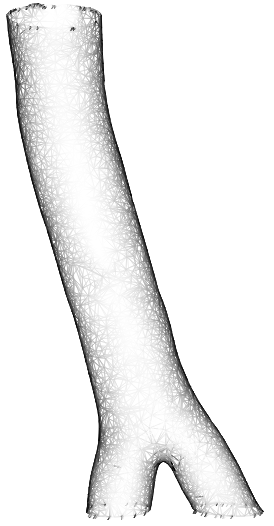
\includegraphics[height=2.0in]{Figures/chap06/smooth_100_01_d90_w.png}%
\label{fig:Decimate90-w}}
\hfil
\subfloat[]{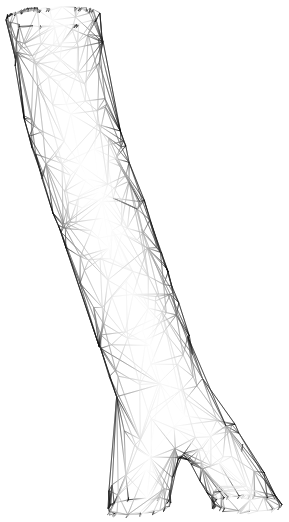
\includegraphics[height=2.0in]{Figures/chap06/smooth_100_01_d99_w.png}%
\label{fig:Decimate99-w}}
\caption{Decimation effects by applying different parameters: top row illustrate the results with reduction rates of $10\%$, $90\%$, and $99\%$, respectively; bottom row illustrate the wire frame representation of the corresponding results depicted above.}%
\label{fig:Decimate}
\end{figure}

In decimating the polygons, the problem is two-folded: on the one hand, the higher rate of reduction is preferred for the following interaction system; on the other hand, however, the over high rate of reduction may lead to heavy tortures on the model surface thus the geometry is doomed to be destroyed. %
This should be taken into consideration when selecting the reduction rate for the decimator algorithm.
In this work, we have tested series of cases with different rates and successfully determined the one that was acceptable in eliminating the excessive polygons.
The output of the decimation process are the progressive meshes \cite{Hoppe1996}.
Besides the aforementioned decimation on the input meshes, the resultant meshes had well preserved the geometry of the model, as well as its global appearance (normals, color values, etc.). %
